\chapter{Lungesykdommer}
		%\chapterprecishere{Vuuuu, vuu vuu\par\raggedleft--- \textup{Molly}, En husky hund fra Drammen}
		\section{Dette har du lært}
			\begin{itemize}
				\item KOLS er underdiagnostisert i Norge.\\
				\item Det er tre spørsmål alle må kunne\cite{anthonisen}:\\
					\begin{itemize}
						\item Hoster du mer enn du pleier?\\
						\item Kommer det opp mer guffe enn vanlig?\\
						\item Er du mer tungpusten enn ellers?\\
					\end{itemize}
				\item KOLS pasienter skal vaksineres.\\
				\item Oksygen er et legemiddel.\\
				\item KOLS pasienter som blir innlagt på sykehus har høy dødelighet.\\
				\item Lavere terskel for antibiotika, for de med KOLS.\\
				\item Blodpropp i lungene er alvorlig og vanskelig å diagnostisere.\\
			\end{itemize}Her presenteres lungesykdommene vi snakker om i kurset. Målet er å lære om KOLS. Forskjellen på KOLS og astma. Lungebetennelse, blodpropp og andre tilstander i lungene beskrives også, men kort.
		\section{Anatomi}
			\paragraph{Stor overflate\\}
				\begin{figure}[ht]
                      \centering
                      	\frame{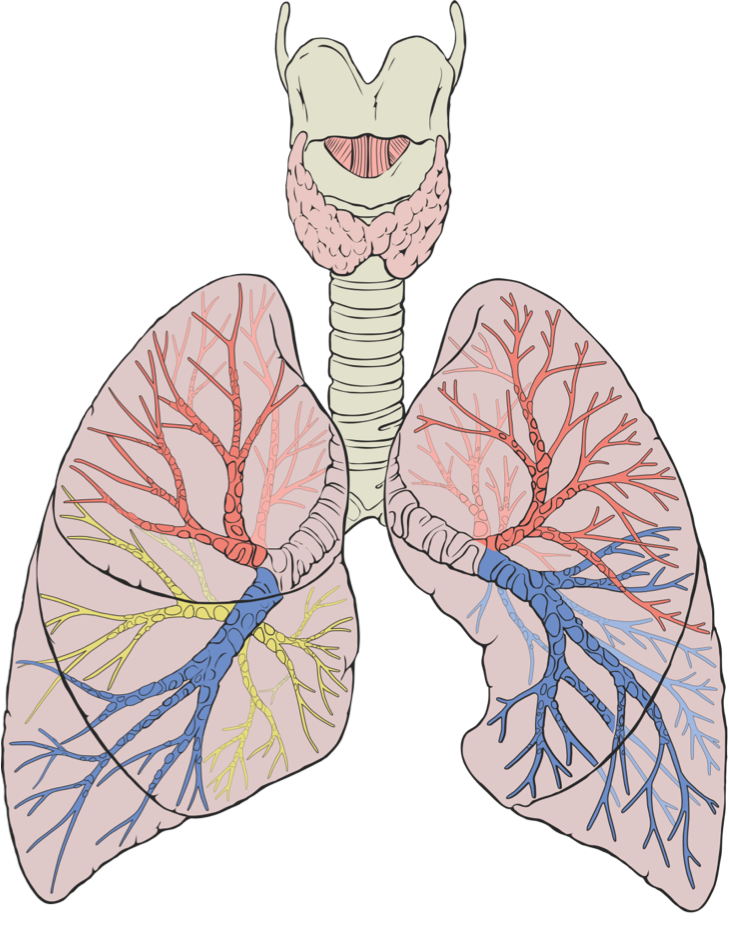
\includegraphics[width=4in]{./kap/bilder/lungeskjema.png}}%!!! må byttes ut, copyright Greys anatomy
                      \caption{Et lungebilde}
                      {Her ser vi et bilde som illusterer lungene og den antomiske oppbygningen}%\textit{tjenestetilbudene}.]
                    \end{figure}
            \paragraph{300 millioner\\}
            	En enorm overflate er nødvendig for effektiv utveksling av oksygen og carbondioksid. Lungene er delt i lapper. Gasutvekslingen finner sted i alveolene(som det finnes 300 millioner av). Lungene har samme overflate som en tennisbane.
		\section{Fysiologi}
				\paragraph{Syre- base\\}
					CO\textsubscript{2} påvirker sammen med bicarbonat syre- base i lungene. Det er en av grunnene til at det tas blodgass av KOLS pasienter. Det kan også bidra til at pasienter med lungesykdommer kan være ustabile.
				\paragraph{Litt om O\textsubscript{2}\\}
					Oksygen kommer inn i kroppen via lungene. Det er ingen andre veier inn. 
		\section{Patologi}
			\paragraph{Arrvev\\}
				Det oppstår arrvev og skader som ødelegger alveolene (emfysem) og obstruksjon av luftveiene hinder luftpassasje i de større luftveiene. Sammen gjør dette at overflaten blir mindre.
			\paragraph{Emfysem\\}
				Konsekvensen av arrvev i lungene kan være store deler av lungen som forsvinner og store hulrom med luft er alt som er igjen. 
					\begin{figure}[ht]
                      \centering
                      	\frame{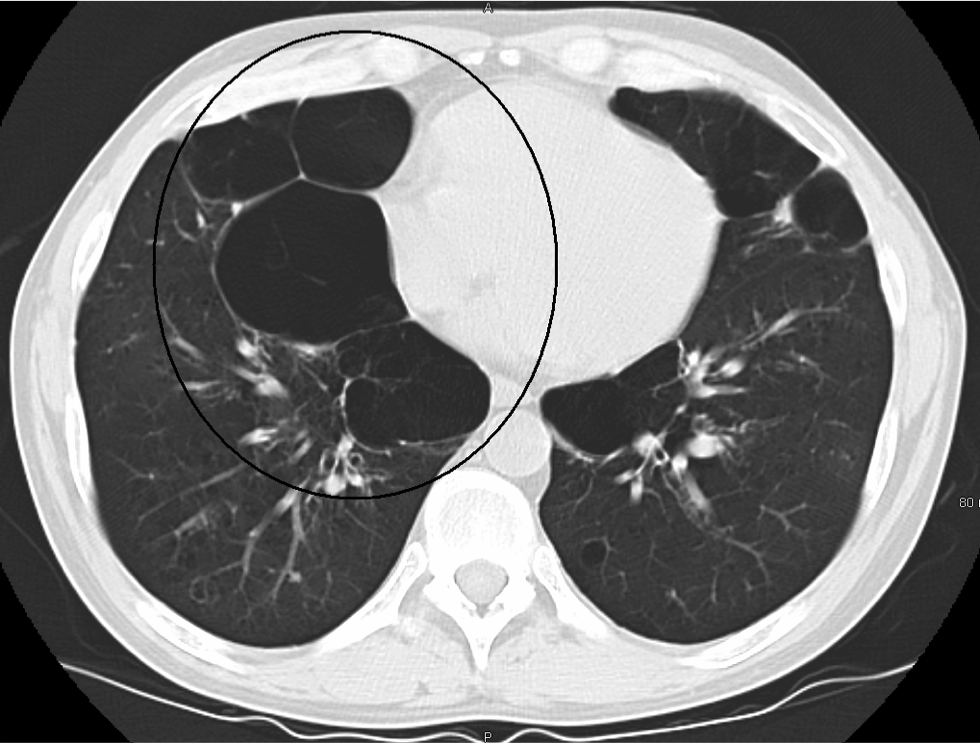
\includegraphics[width=5in]{./kap/bilder/emfysemct.png}}%!!! må byttes ut, copyright Greys anatomy
                      \caption{Et CT-bilde av en emfysemlunge}
                      {Her ser vi et CT-bilde av lunger med emfysem. Dette er ikke alltid mulig å se på vanlig røntgen. Det samme gjelder med ultralyd.}%\textit{tjenestetilbudene}.]
                    \end{figure}
            \paragraph{Andre problemer\\}
            	Mange andre tilstander påvirker lungefunksjonen. Dette er ikke en fullstendig liste men: pneumothoraks, pleuravæske, lungebetennelser, lungeødem, lungearterieemboli og mange flere. Ofte er sykdomstilstanden kjent, men det er viktig å huske på at for eksempel KOLS pasienter har hyppigere pneumothoraks enn den vanlige befolkningen. Lærepoenget er at vi skal huske på at vi må gjøre diagnostikk, selv på velkjente KOLS pasienter med forverringer. 
		\section{Klinikk}
			\subsection{KOLS}
				\paragraph{Største pasientproblemer\\}
					Tungpust er det største hinderet i hverdagen. For mange er belastningen med røykeslutt også en vanskelig byrde med sosiale konsekvenser. 
				\paragraph{Mange viktige målinger\\}
					Spirometri gir diagnosen KOLS. Klassifiseringen er GOLD, stadium I-IV, hvor IV er mest alvorlig.
						\begin{figure}[ht]
                      \centering
                      	\frame{
\includegraphics[width=6in]{./kap/bilder/goldnorsk.png}}%!!! må byttes ut, copyright GOLD
                      \caption{GOLD klassifiksjonen}
                      %{Her ser vi et bilde som illusterer lungene og den antomiske oppbygningen}%\textit{tjenestetilbudene}.]
                    \end{figure}
			\subsection{Pneumoni}
				Infeksjoner i lungene er veldig vanlig. Vanligvis kan dette behandles med penicillin, men ikke hos KOLS pasienter. Symptomer er: Feber, slapphet og produktiv hoste. Det er ikke uvanlig med septiske forløp hos eldre. 
			\subsection{Lungeemboli}
				Blodpropper fra beina blir fanget i lungene dersom de løsner. Pasienter kan ha forkjellige symptomer, som tungpust, pusteavhengige smerter, smerter i brystet eller andre diffuse plager. Problem: Alle symptomene kan passe til andre sykdommer også.
		\section{Pasienteksempler}
			\subsection{Pasient 5}
			\subsection{Pasient 6}